% Die Beamer-Klasse unterstützt folgende Optionen, die von
% besonderem Interesse sind (alle Standardoptionen werden
% ebenfalls unterstützt; siehe beamer-Basisdokumentation):
% 
%%%%%%%%%%%%%%%%%%%%%%%%%%%%%%%%%%%%%%%%%%%%%%%%%%%%%%%%%%%%%%%
% aspectratio: Seitenverhältnis des resultierenden Dokuments
% (Achtung: Aufgrund der Designvorgaben ergeben sich unterschiedliche
% Größen der effektiv nutzbaren Textblöcke)
%
% Standardeinstellung: 'aspectratio=43'
%
% Mögliche Einstellungen:
% 'aspectratio=43'   (4:3)
% 'aspectratio=169'  (16:9)
% 'aspectratio=1610' (16:10)
% 
%%%%%%%%%%%%%%%%%%%%%%%%%%%%%%%%%%%%%%%%%%%%%%%%%%%%%%%%%%%%%%%
% fontsize: Basisschriftgröße (Größen für Überschriften etc. werden
% aus dieser Basis automatisch abgeleitet)
%
% Standardeinstellung: '22pt' (entspricht den Design-Vorgaben; sehr groß!)
%
% Mögliche Einstellungen:
% '8pt', '9pt', '10pt', '11pt', '12pt', '14pt', '16pt',
% '17pt','20pt','22pt', '24pt', '26pt', '28pt'


\documentclass[aspectratio=169,16pt]{beamer}

% Der OTHR-Theme unterstützt folgende Optionen:
% 
%%%%%%%%%%%%%%%%%%%%%%%%%%%%%%%%%%%%%%%%%%%%%%%%%%%%%%%%%%%%%%%
% department: (Wahl der Abteilung/Fakultät)
%
% default: 'OTHR'
%
% Mögliche Einstellungen:
% 'FakA', 'FakAM', 'FakB', 'FakBW', 'FakEI', 
% 'FakIM', 'FakM', 'FakS', 'ZWW', 'IPF',
% 'SappZ', 'KNB', 'ReMIC', 'LFD', 'LAS3',
% 'DK0PT', 'LBM', 'LeanLab', 'LFT', 'LFW',
% 'LMP', 'LMS', 'LRT', 'LWS', 'RRRU',
% 'RST', 'CEEC', 'FEM', 'IST'
%%%%%%%%%%%%%%%%%%%%%%%%%%%%%%%%%%%%%%%%%%%%%%%%%%%%%%%%%%%%%%%%%
% headerMode: Aussehen und Inhalt der Kopfleiste
%
% Standardeinstellung: 'full'
%
% Mögliche Einstellungen:
% 'full', 'frametitle', 'frametitleSection'
% 

%%%%%%%%%%%%%%%%%%%%%%%%%%%%%%%%%%%%%%%%%%%%%%%%%%%%%%%%%%%%%%%%%
% Binäre Schalter (können angegeben oder nicht angegeben werden;
% Standardeinstellung: Nicht angegeben)
%
%%%%%%%%%%%%%%%
% navbar: Navigationssymbole anzeigen (Seite vor/zurück, Kapitel vor/zurück etc.)

% pageNumbers: Seitennummerierung

% blackFont: Nur schwarze Schriftfarbe verwenden (ansonsten: Fakultätsfarben)

% frametitleCenter: Titel in der Kopfzeile zentrieren (ansonsten: rechtsbündig)

\usetheme[department=FakIM,pageNumbers]{OTHR}

% Inhaltsspezifische Zusatzpakete laden 
\usepackage[ngerman]{babel}
\usepackage[utf8]{luainputenc}

\useDepartmentLogo

\begin{document}

\title{URL shortener on Google Cloud}
\author{Dennis Bejze}
\institute{Faculty of Computer Science and Mathematics}
\date{31th May 2022}

\maketitle

\frame{\frametitle{Agenda}\tableofcontents}

\section{What is a URL shortener?}

\begin{frame}
    \frametitle{How does it work?}

    \begin{itemize}
        \item Its task is to provide a shortened URL for a longer one
        \item If the user eventually visits the shorter URL, he or she will be redirected to
              the webpage of the longer URL
              \begin{itemize}
                  \item It's like making a kind of alias for a desired URL
                  \item Makes it more readable
              \end{itemize}
    \end{itemize}
\end{frame}

\section{Cloud integration}

\subsection{Development environment}
\begin{frame}
    \frametitle{Programming languages and technologies}
    \begin{columns}[onlytextwidth]
        \begin{column}{0.65\textwidth}
            \begin{description}
                \item [Server-side:]Go
                \item [Client-side:]React with TypeScript
            \end{description}
        \end{column}
        \begin{column}{0.35\textwidth}
            \vspace{-2em}
            \begin{figure}
                
\includegraphics[height=.3\paperheight]{Go-Logo_Blue}
                
\includegraphics[height=.3\paperheight]{React-Logo}
            \end{figure}
        \end{column}
    \end{columns}
\end{frame}

\subsection{Used cloud services}
\begin{frame}
    \frametitle{How did the project benefit from the cloud services?}

    \begin{columns}[onlytextwidth]
        \begin{column}{0.5\textwidth}

            \begin{itemize}
                \item Cloud Run (hosts containerized applications)
                      \begin{itemize}
                          \item Web application inside of Docker container (practical, because for such a simple
                                application a whole VM was not necessary)
                      \end{itemize}
                \item API Gateway (brings together multiple backend services)
                      \begin{itemize}
                          \item Single, clear point of interaction with business logic
                          \item Made it easier to design an API with different backend services (flexible)
                      \end{itemize}
            \end{itemize}

        \end{column}%
        \begin{column}{0.5\textwidth}
            \begin{center}
                \begin{figure}
                    \centering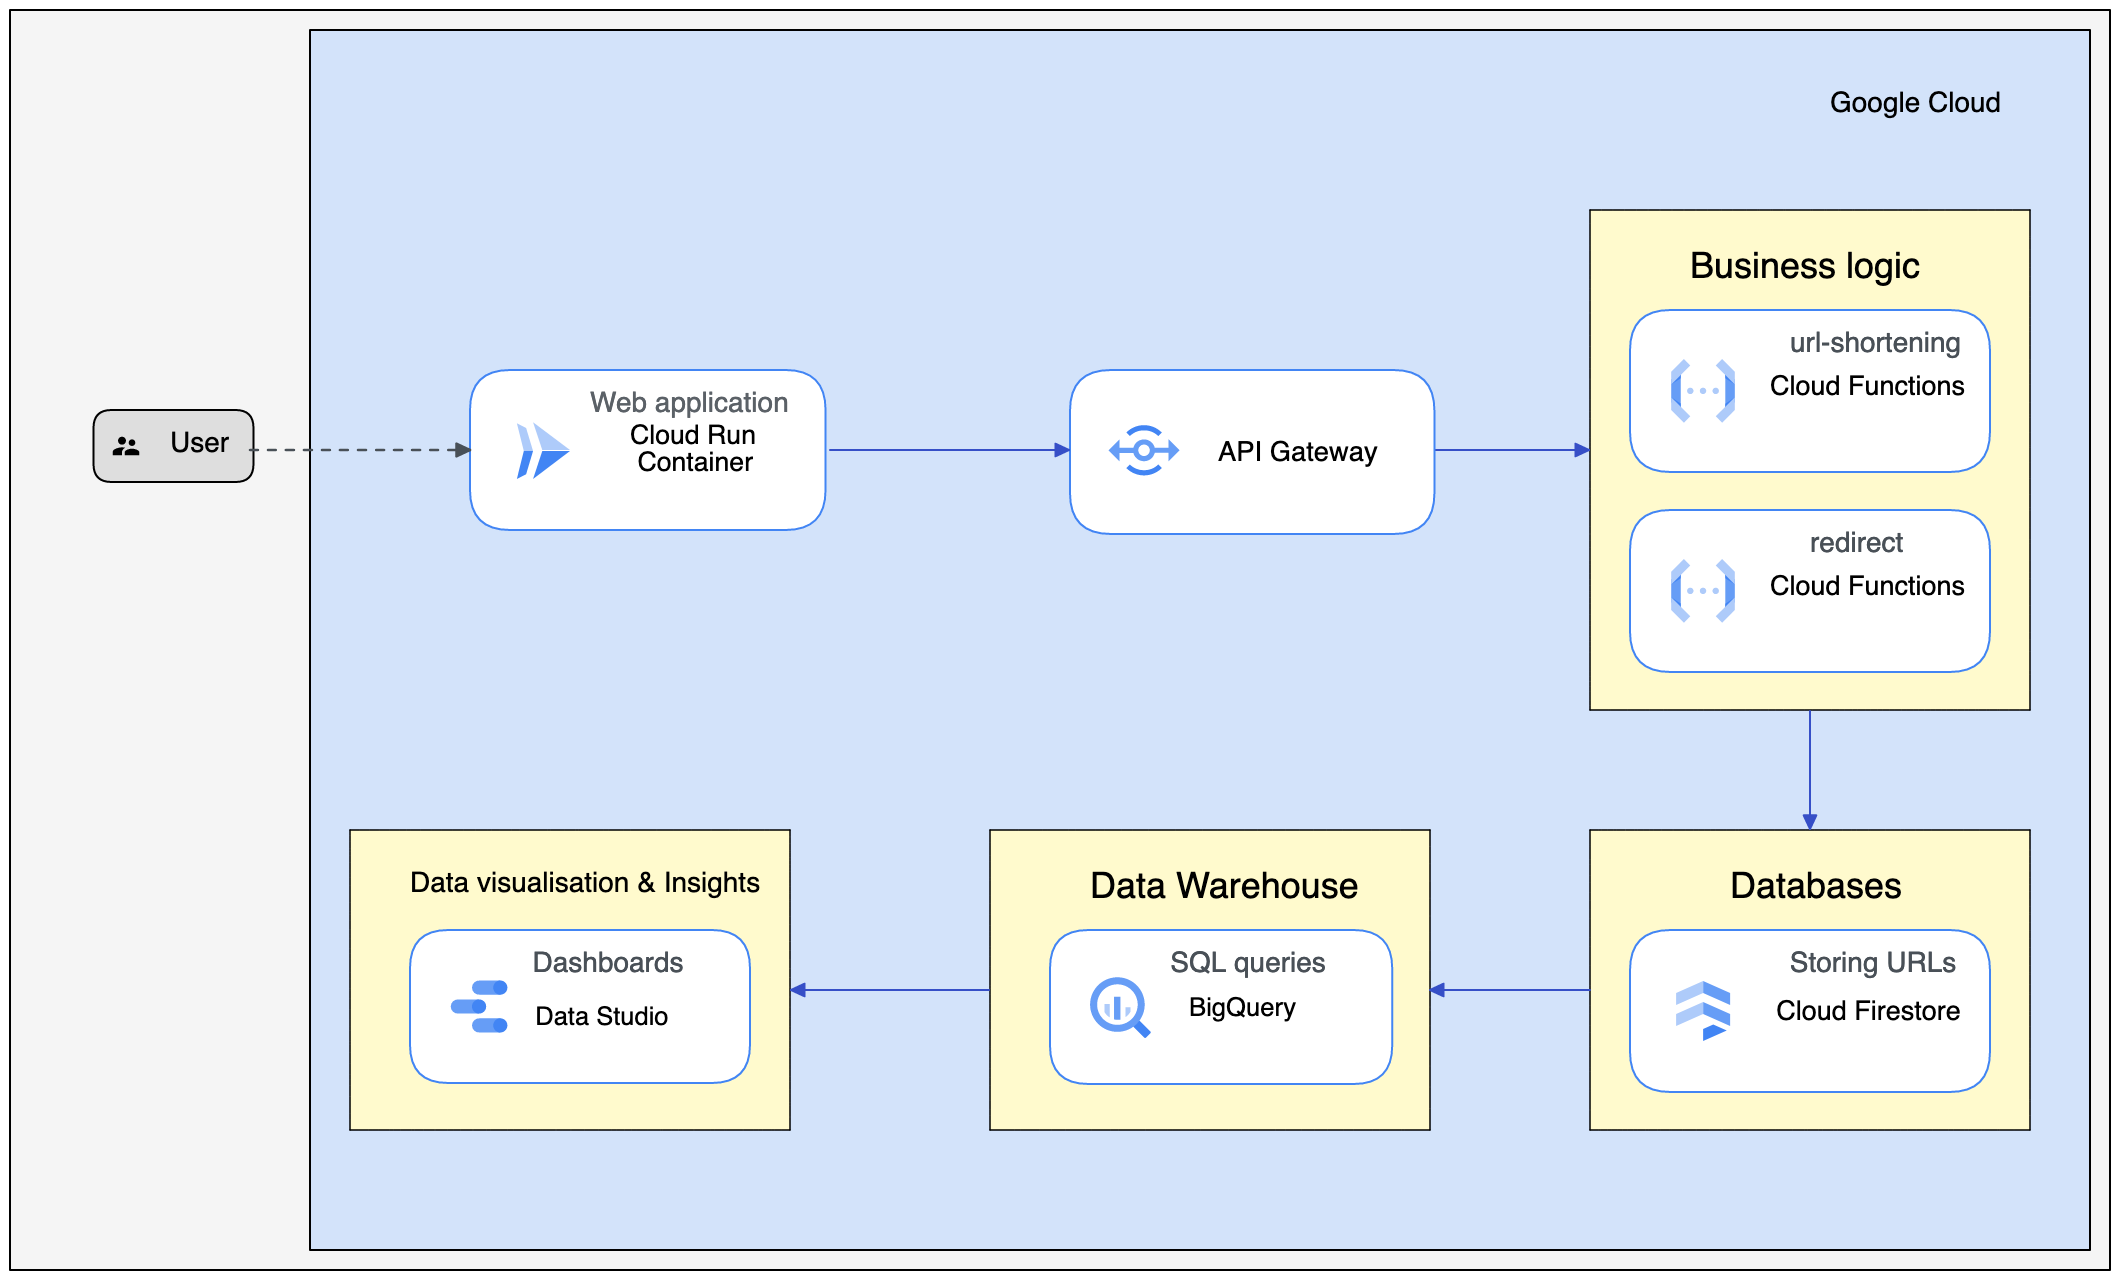
\includegraphics[height=.5\paperheight]{architecture}
                \end{figure}
            \end{center}
        \end{column}
    \end{columns}
\end{frame}

\begin{frame}
    \frametitle{How did the project benefit from the cloud services?}

    \begin{columns}[onlytextwidth]
        \begin{column}{0.5\textwidth}

            \begin{itemize}
                \item Cloud Functions (simple, single-purpose functions)
                      \begin{itemize}
                          \item Serverless functions were ideal for the simple logic of shortening and redirecting
                      \end{itemize}
                \item Firestore (NoSQL database)
                      \begin{itemize}
                          \item NoSQL, because the 'tuples', containing a long and the corresponding shorter URL,
                                are just simple objects
                          \item Avoided creating unnecessarly complex relations (tables)
                      \end{itemize}
            \end{itemize}

        \end{column}%
        \begin{column}{0.5\textwidth}

            \begin{center}
                \begin{figure}
                    \centering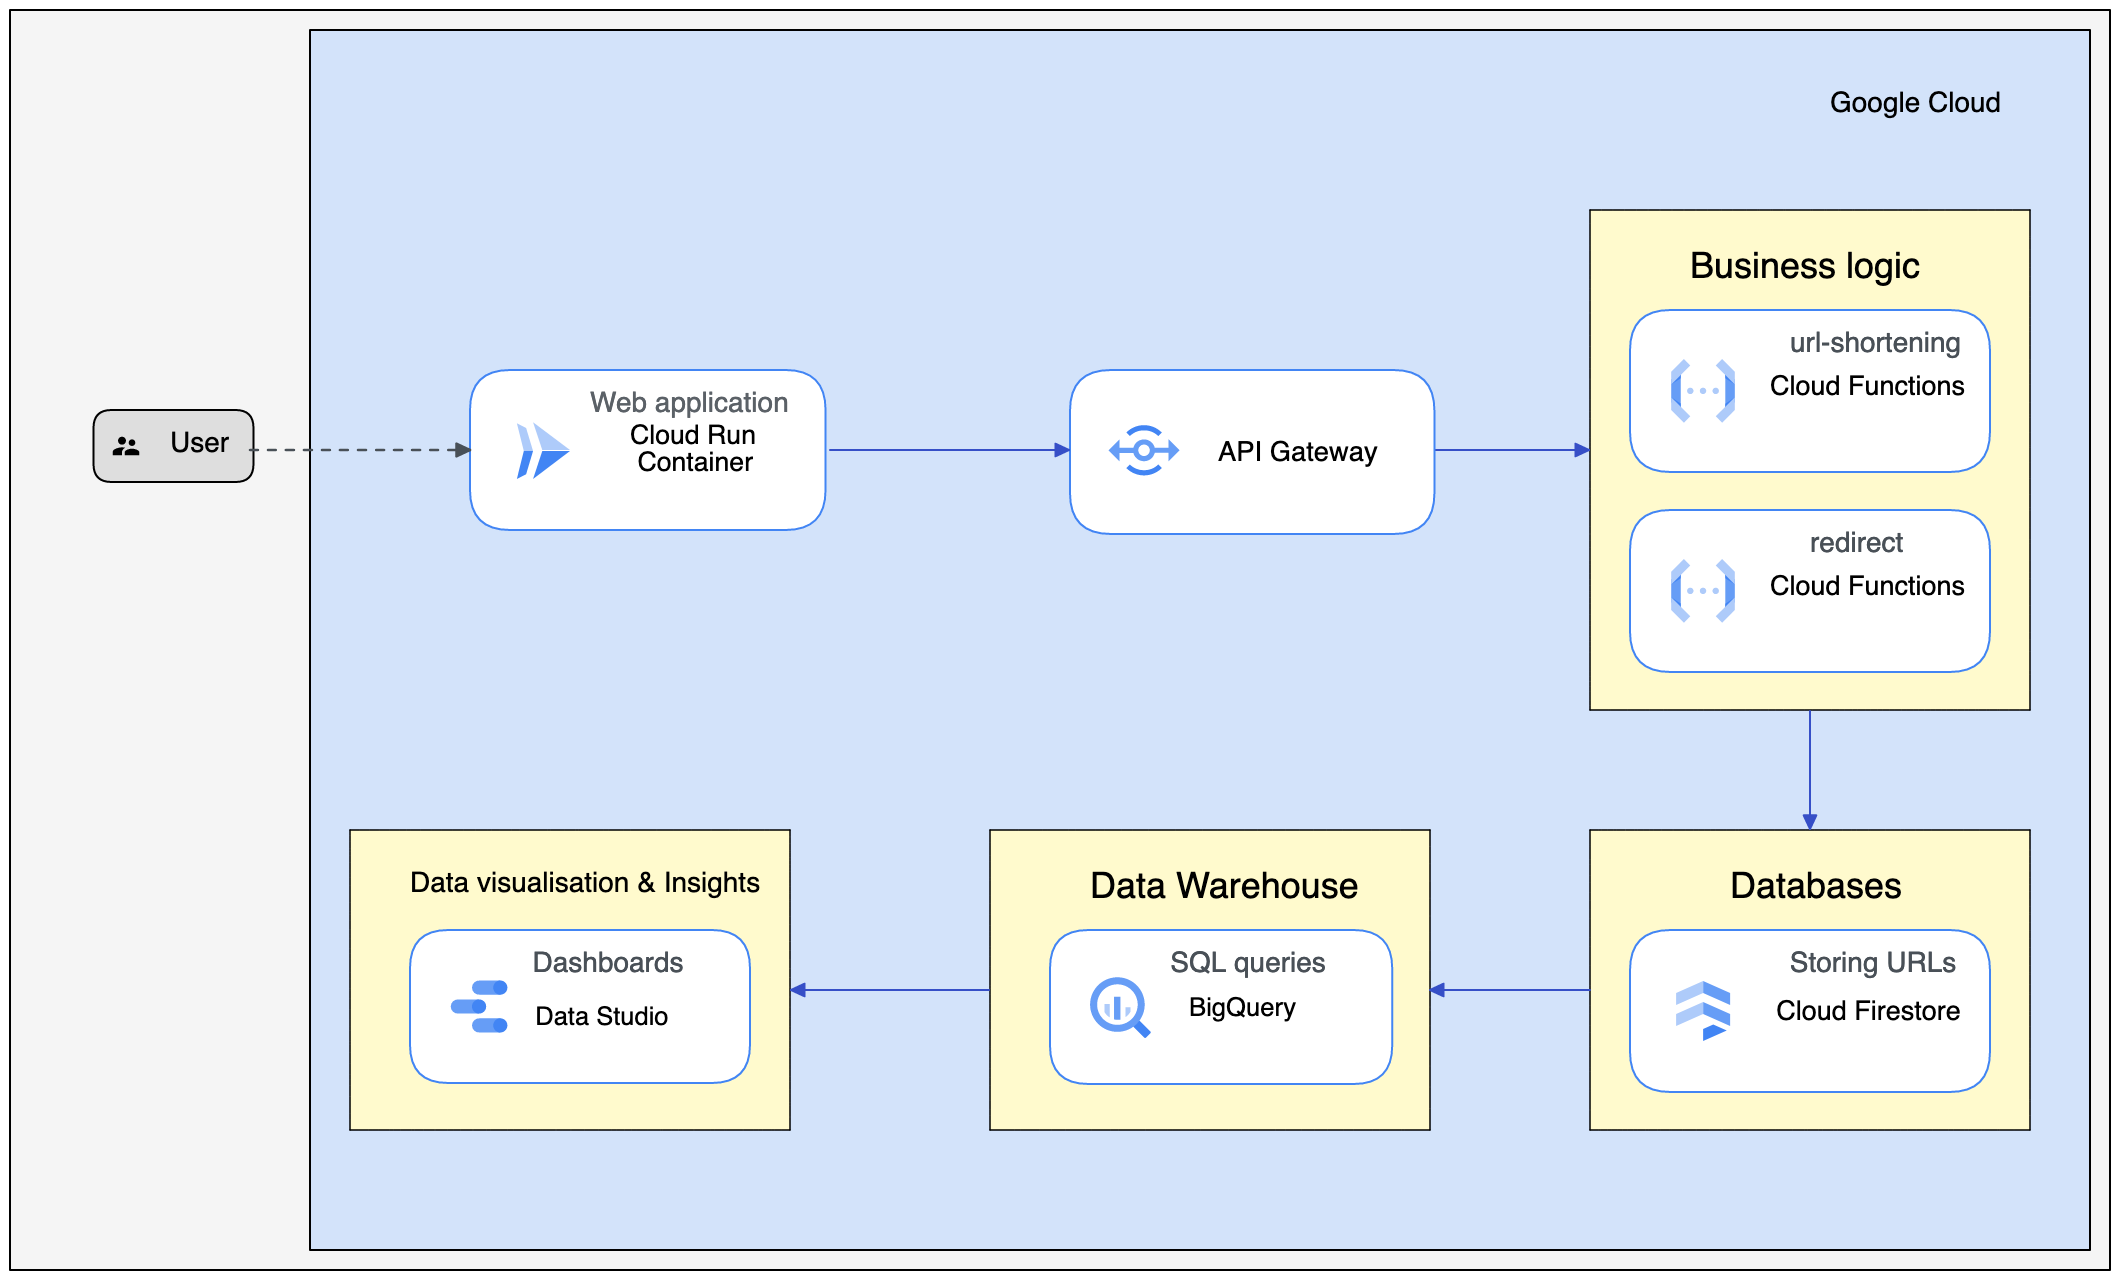
\includegraphics[height=.5\paperheight]{architecture}
                \end{figure}
            \end{center}

        \end{column}
    \end{columns}
\end{frame}

\begin{frame}
    \frametitle{How did the project benefit from the cloud services?}

    \begin{columns}[onlytextwidth]
        \begin{column}{0.5\textwidth}
            \begin{itemize}
                \item BigQuery (data warehouse)
                      \begin{itemize}
                          \item Import function made it possible to not go completely without
                                'traditional' SQL
                          \item Convenient to analyze data
                      \end{itemize}
                \item Data Studio (Visualization of data)
                      \begin{itemize}
                          \item Connection can be easily established between BigQuery data source
                                and the diagrams
                      \end{itemize}
            \end{itemize}
        \end{column}

        \begin{column}{0.5\textwidth}

            \begin{center}
                \begin{figure}
                    \centering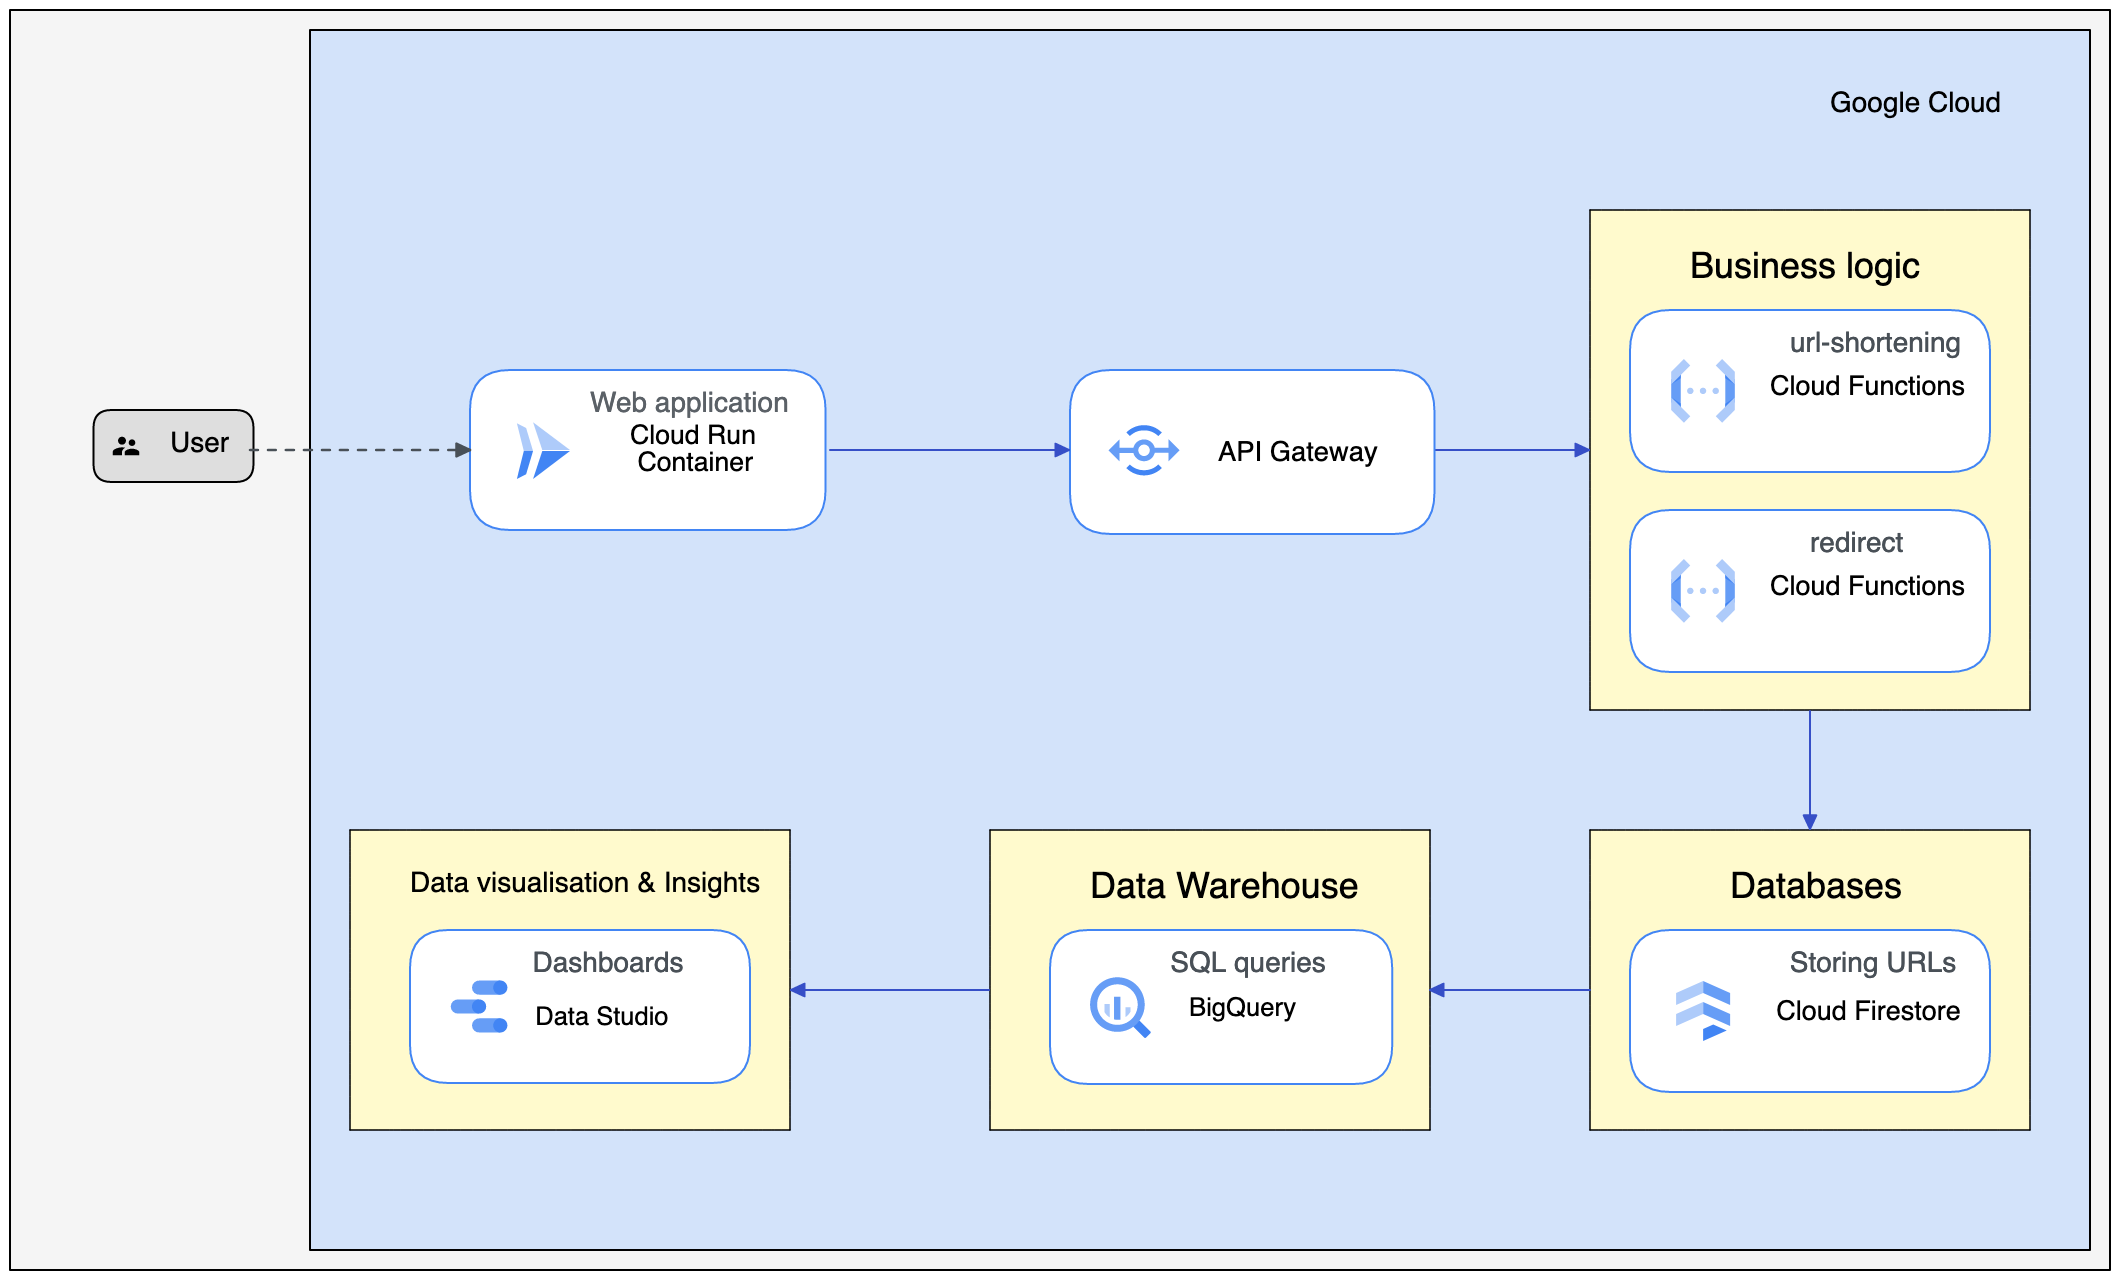
\includegraphics[height=.5\paperheight]{architecture}
                \end{figure}
            \end{center}

        \end{column}
    \end{columns}
\end{frame}

\section{Demonstrating the URL shortener}
\begin{frame}
    \frametitle{Web application}
    \begin{block}{\scriptsize My application can be found at:} \scriptsize
        \href{https://shortenyoururl-f7gnpjx2ea-ey.a.run.app/}{https://shortenyoururl-f7gnpjx2ea-ey.a.run.app/}
    \end{block}
\end{frame}

\begin{frame}
    \frametitle{Example of one of my cloud service dashboards}
    \begin{figure}
        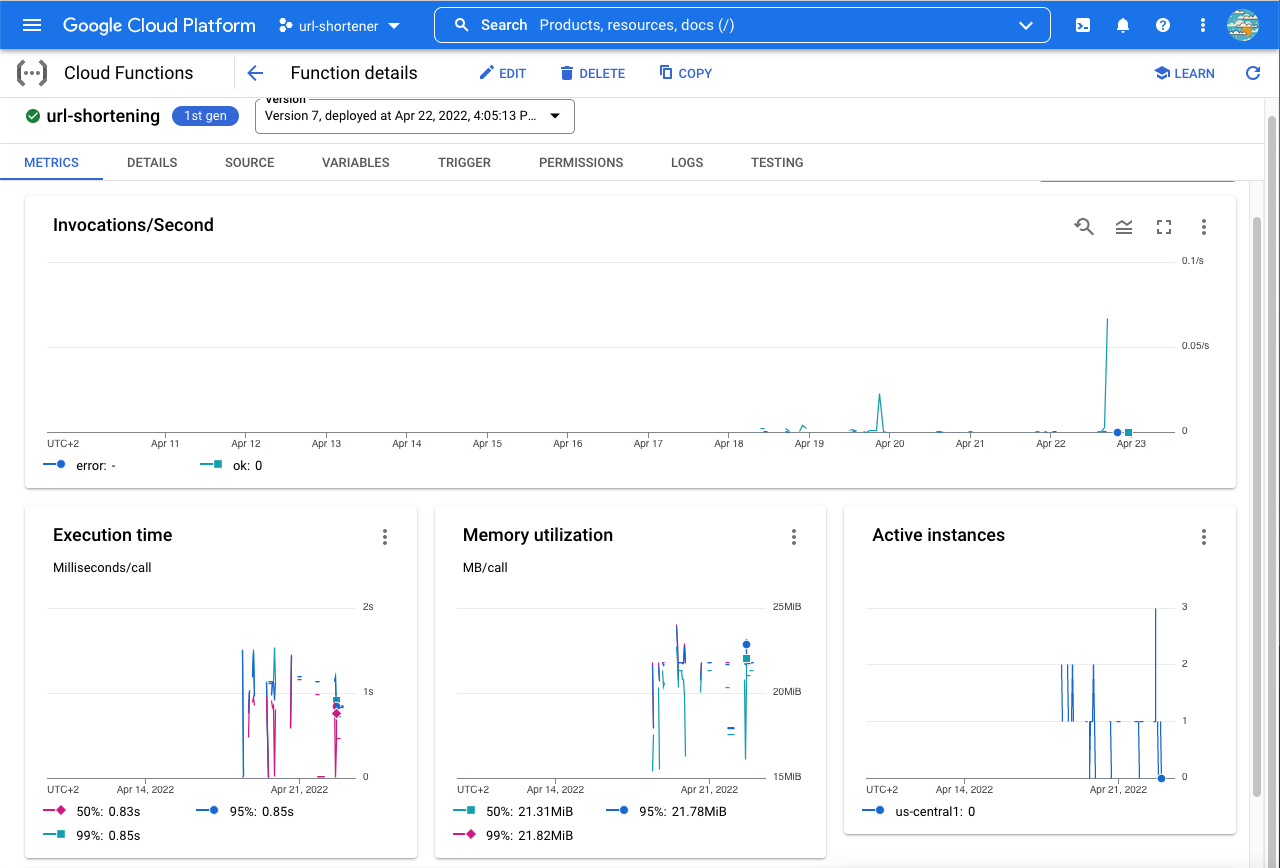
\includegraphics[height=0.75\paperheight]{cloudFunctionDashboard}
    \end{figure}
\end{frame}

\begin{frame}
    \frametitle{Dashboard in Data Studio}
    \begin{figure}
        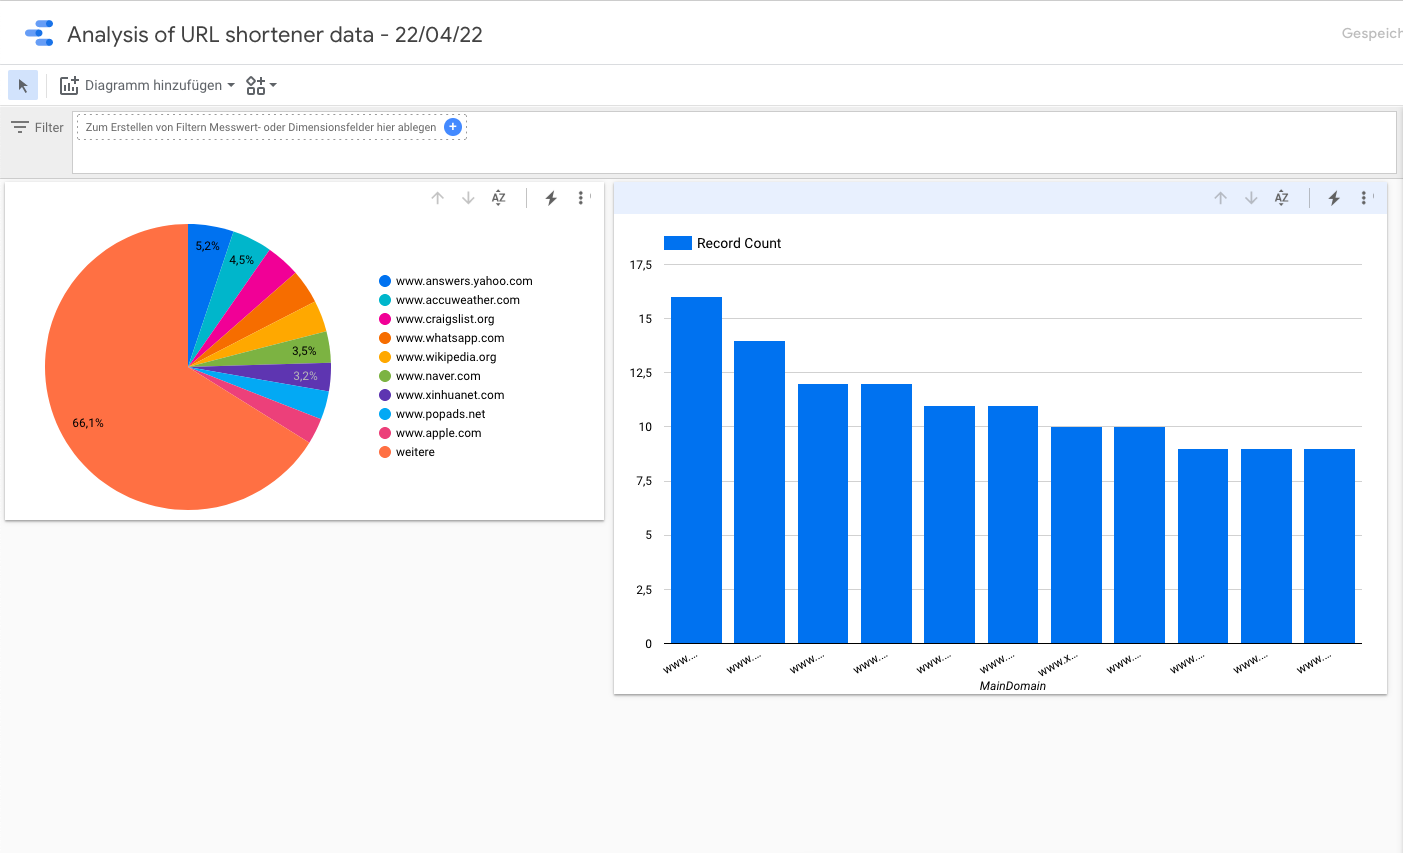
\includegraphics[height=0.75\paperheight]{dataStudioDashboard}
    \end{figure}
\end{frame}

\section{Impressions and feedback of using the cloud}

\begin{frame}
    \frametitle{Impressions and Feedback}

    \begin{block}{\scriptsize First impressions}
        \begin{itemize} \scriptsize
            \item Amazed, how many services Google Cloud were offering
            \item Cloud Console was a bit overwhelming in the beginning
        \end{itemize}
    \end{block}

    \begin{block}{\scriptsize Feedback}
        \begin{itemize} \scriptsize
            \item It was pleasant to have such generously designed quotas - learning
                  and prototyping is made convenient for beginners
            \item Google Cloud has well written documentation for their different services
                  \begin{itemize}
                      \item Especially the quickstarts were always useful as a starting point
                  \end{itemize}
        \end{itemize}
    \end{block}
\end{frame}

\begin{frame}[allowframebreaks,nosection]
    \frametitle{Sources}
    \begin{itemize} \tiny
        \item Go Logo (n.d.), https://go.dev/blog/go-brand [Online; visited on 22/04/22]
        \item React Logo (n.d.), https://commons.wikimedia.org/wiki/File:React-icon.svg [Online; visited on 22/04/22]
    \end{itemize}
\end{frame}

\begin{frame}[allowframebreaks,nosection]
    \begin{center}
        \huge Thank you for your attention!
    \end{center}
\end{frame}

\end{document}
